% Focused manuscript. Recovery results input is finalized by the lead integrator.
\RequirePackage[T1]{fontenc}
\documentclass[conference]{IEEEtran}
\usepackage{amsmath,amssymb}
\usepackage{newtxtext,newtxmath}
\usepackage{graphicx}
\graphicspath{{paper/figures/}{figures/}}
\usepackage{booktabs,array}
\usepackage{seqsplit}
\usepackage{balance}
\usepackage{placeins}
\usepackage{url}
\usepackage[hidelinks]{hyperref}
\urlstyle{same}
\title{ConseqaX: An Evidence Protocol for Recovering Ambiguous Agent Actions}
\author{\IEEEauthorblockN{Devrajsinh Jhala}\IEEEauthorblockA{Independent Researcher}}
\begin{document}
\raggedbottom
\maketitle

\begin{abstract}
A timed-out tool call can leave an agent uncertain whether an operation failed or will commit later. ConseqaX separates state, action-origin and unknown conclusions through explicit contracts and readback witnesses. Study A retains 15,360 SQLite worlds from 24 authored cases: readback safely recovers 14/24 versus 8/24 for response-driven retry, matching a strong reference. Repeated seeds add no recorded-metric diversity; polling adds no coverage and detection does not repair all harmful effects. Study B retains 960 worlds: polling raises correct-state yield from 3/192 to 81/192 at 741 versus 192 reads, with identical physical outcomes. The externally authored LIMBO study covers 12 base instances, 24 task/fault conditions and four arms. The interrupted original retains 6/96 audited grades. A separately declared follow-up, after partial-data exposure, retains another 96 planned slots on the same instances; cohorts are not pooled. Replay establishes 96/96 follow-up grades, including 3 native error returns after settlement. All-planned results are Vanilla: TS 21/24, EOS 16/24; SDK retry: TS 24/24, EOS 14/24; Native guard: TS 21/24, EOS 16/24; ConseqaX guard: TS 20/24, EOS 15/24. The package emits 3 audited receipts in 3/24 episodes, with complete accounting in 24/24. Receipt activation demonstrates integration rather than a new recovery algorithm. Missing grades remain unavailable. Native EOS has domain-specific accounting, not a universal exactly-once guarantee. Study A's packaging deviation remains disclosed. These finite simulator results establish neither task-population superiority nor independent service validation.
\end{abstract}
\begin{IEEEkeywords}agent systems, outcome verification, recovery, idempotency, evidence provenance, uncertainty\end{IEEEkeywords}

\section{Introduction}

An agent requests an inventory allocation, ticket, or published artifact. The provider accepts the operation, but the acknowledgement times out. An immediate retry may create a second record; stopping may leave the task unfinished. A separate read can reveal an existing effect, yet even a fresh empty snapshot cannot establish that the first request will never commit later. A reliable recovery decision depends on the operation's identity, provider guarantees, temporal target, and available evidence, rather than the response alone.

Three distinctions matter. First, a response describes a tool interaction, whereas a readback supplies evidence about external state. Second, global task satisfaction differs from an effect being linked to this agent's operation. Another actor can complete the task; missing actor metadata need not imply an external actor. Third, a hindsight-correct assertion can have been unsupported when issued. A controller that guesses the eventual outcome correctly has not thereby justified a retry or a completion claim.

These are established systems and verification concerns \cite{helland,vogels,verified,operability,agenttool,limbo}. ConseqaX makes them explicit in a reusable evidence protocol \cite{artifact}. Its typed records bind contracts, attempts, responses, observations, and verification receipts. Admitted readback can support satisfied, violated, or unknown state, while origin remains a separate conclusion. The protocol does not authenticate a provider or manufacture request finality. Applications supply source semantics and the policy connecting receipts to actions.

This paper centers that policy boundary. We compare response-driven same-key retry, state-only readback, a separately implemented provenance-aware reference, a package-backed single-final-read ablation, and package-backed bounded polling. Controller actions change subsequent SQLite effects and observations. The experiment asks whether the declared evidence policy changes safe recovery, final-report correctness, or definite-report coverage at a measured read/wait cost, and when ordinary provider idempotency removes the apparent advantage.

The research questions are falsifiable. \textbf{Q1:} How does polling change safe recovery relative to response-driven retry, together with own harmful effects and recovery failures? \textbf{Q2:} Does the package-backed implementation agree with a same-information reference using separate evidence arithmetic? \textbf{Q3:} What additional origin-report coverage and correctness appear beyond state-only reporting? \textbf{Q4:} Does continued polling change final-report correctness and coverage relative to one final read at its additional resource cost? \textbf{Q5:} What abstention and definite-error tradeoffs remain under incomplete public histories? Equal or worse recovery, incorrect conclusions, unnecessary reads, or parity under shared provider guarantees can limit the proposed benefit. \textbf{Q6:} Under native ambiguous-commit faults, how do all-planned task/effect outcomes, failures and actual work differ among vanilla dispatch, transparent retry, the supplied strong guard and its receipt-preserving SDK integration?

The contributions are an executable evidence protocol, a controlled evaluation of recovery/reporting boundaries and a native external fault-benchmark integration with audited first-attempt accounting. The controlled reference uses separate arithmetic but shares application transitions; its agreement supports conformance. The external SDK arm deliberately preserves an established strong guard, so it does not introduce a new recovery algorithm. Provenance changes only reporting in the controlled shared-transition comparison. The native experiment and actual results in Sections~\ref{sec:limbo} and~\ref{sec:limbo-results} retain 96 planned slots per cohort on the same 12 base instances, including the original interrupted cohort and the separately frozen follow-up. Neither repeated seeds nor repeated arms create independently sampled tasks.

\section{Related Work and Positioning}

Idempotence and eventual consistency are longstanding systems concerns \cite{helland}, \cite{vogels}. Verified Tool Calls separates acknowledgements from independently checked effects and admits unknown postconditions \cite{verified}. Callability Is Not Operability examines controlled interface ambiguity and terminal agent claims \cite{operability}. Agent-tool anomaly work distinguishes runtime observations from external events \cite{agenttool}. LIMBO grades committed-effect histories and studies late commits \cite{limbo}. Consequently, response/effect separation, effect ledgers, and the danger of ambiguous retries are foundations and comparison requirements here, rather than priority claims.

PROV-DM represents entities, activities, agents, and responsibility \cite{prov}. ConseqaX is neither a new general provenance model nor a PROV conformance implementation. Its narrower boundary links operation identity, temporal contracts, individual observation witnesses, and explicit unknown verdicts. A source-supported origin link is not proof that the action was counterfactually necessary.

Causal Agent Replay (CAR) performs same-policy interventions with contrastive suffix and permutation Shapley attribution \cite{car}. Policy-Conditioned Counterfactual Credit studies verified outcomes under declared interventions and continuation policies \cite{pccc}; CausalLoss-Fin jointly intervenes on decisions and infrastructure messages \cite{causalloss}. Those questions differ from whether a live recovery action is justified by its available evidence. Our earlier replay adapter uses existing estimators. The present experiment requires neither counterfactual writes nor a new attribution method.

AppWorld, ToolSandbox and tau-bench evaluate stateful agent interaction and world outcomes \cite{appworld,toolsandbox,taubench}. Earlier model-free transfer used maintained retail/airline tools and native DB evaluation \cite{tau3tasks,tau3eval}; reference-action replay is not an autonomous score. Our external experiment uses LIMBO's authored tasks, native faults and unchanged grader \cite{limbo,limbosource}, retaining its supplied strong guard as a comparator. The receipt arm tests protocol integration under that same recovery law. The native grade and independently replayed effect history extend the controlled evaluation while remaining simulated evidence from one local quantized model.

The present contribution is therefore conditional: an executable evidence contract and an auditable comparison of policy tradeoffs under declared capabilities. Its value must come from the recovery behavior, final-report correctness, coverage, and cost actually measured, rather than from attributing established distributed-systems guarantees to a framework.

\section{Evidence and Recovery Protocol}

This section specifies the temporal record contract and application recovery law evaluated in controlled Studies A and B. The external LIMBO condition instead uses the benchmark's own guard and a custom current-public-report verifier; it does not apply this controller or the temporal RecordVerifier to native reports.

\subsection{Objects and temporal targets}

A logical action has stable identity and payload; each dispatch has a distinct attempt identity. Captured records include the request, provider response, reported assessment, separately captured observation, and resulting verification receipt. Reported assessments are outputs, not measurements of hidden reasoning. An observation states its source, scope, completeness, availability, observation time, watermark, and effect history. The application declares which source and clock are authoritative.

Let registration be $t_0$, the original deadline $D$, stability duration $W$, and original horizon $H=D+W$. The original contract remains fixed. A separate recovery deadline $R\geq H$ and safety horizon $S\geq R$ define later recovery in this study: its matching candidates must commit by $R$ and persist through $S$, and its count is checked throughout $[R,S]$. A later completion may satisfy recovery while violating the original SLA. Neither a new read nor an explanatory receipt moves $D$.

For the exact-count record contract, a candidate matches the expected business fields, commits within $[t_0,D]$, and persists through $H$. The declared count must hold, including the maximum simultaneous matching count over $[D,H]$. Historical removals and transient extras therefore matter; a current-row snapshot alone is insufficient. Simultaneous commits and removals are evaluated together, with boundary conventions fixed before collection.

The verifier concludes satisfied, violated, or unknown. A complete admitted observation must cover the registered scope and history through $H$. Stale watermarks, inadequate scope, unavailable reads, or malformed history retain unknown. Source identity, completeness, timestamps, and provenance are trusted adapter declarations. Schema checks and hashes establish structure and retained bytes, not source authenticity or transactional guarantees.

\subsection{State, origin, and support}

Global state satisfaction does not require this agent to have produced the effect. Action-linked satisfaction additionally requires qualifying target evidence linked to the logical operation. A known global violation makes this linked contract false even if an own matching record exists: a second effect can invalidate an exactly-one task. Mere witness presence cannot replace the whole contract.

A matching action identity with absent or matching actor metadata can support linkage under the admitted provenance law. Explicitly different identities exclude this operation; missing or conflicting linkage can remain unknown. Provenance does not turn an externally satisfied state into a failure. Each observation retains its own witnesses. A later record sharing an effect ID cannot inherit an earlier observation's origin link while silently changing payload, actor, or removal history.

Hindsight correctness and evidence support are distinct questions. The controlled-study evaluator scores final state and action-linkage reports against full-ledger truth, with separate definite-report and abstention counts. It does not independently label support at issuance or score safe-to-retry assertions. Retained public histories permit automated checks against the declared admission rules; a hindsight-correct guess alone does not establish support. An origin abstention does not erase a definite state conclusion. Conditional error among definite assessable reports and correct definite yield over all planned worlds answer different questions.

\subsection{Why historical absence cannot resolve a pending attempt}

\textbf{Conditional retry boundary.} Suppose an operation times out without atomic deduplication, terminal resolution, completed cancellation, or an enforceable in-flight bound. Let $L<R$ be the last useful retry time. Two provider worlds give identical admissible histories through $L$: the initial attempt never commits in one and commits after $R$ but by $S$ in the other. A retry by $L$ achieves recovery by $R$; a later retry cannot. An extra effect is harmful even if compensated, and no alternative operation achieves the target.

A deterministic policy takes the same decision in both histories. Retrying creates a duplicate in the late-commit world; declining misses recovery in the never-commit world. For a randomized policy, couple its randomness and let $p$ be its useful-retry probability. Duplicate risk in the second world is at least $p$ and missed-recovery risk in the first at least $1-p$. Their sum is at least one for this constructed pair. This elementary indistinguishability argument states a known systems boundary \cite{limbo}, rather than a new impossibility or a measured prevalence. Provider guarantees can break its assumptions.

\subsection{Application safety gate and bounded reads}

Every policy preserves the operation key and payload. When a public native idempotency capability is admitted, the provider atomically reserves pending and completed work for that key. All readback policies may use the same-key exception to retry within the common cap before $D$. The response-driven arm also benefits from the identical provider semantics; it is the ordinary bounded idempotent-retry comparator in that stratum.

Without that capability, the readback policies permit another dispatch only when every previous attempt has an admitted terminal-no-effect guarantee, fresh complete trusted readback establishes no relevant effect through the decision time, budget remains, and time is strictly before $D$. A newer terminal response does not resolve an older ambiguous request. An empty watermark proves only past absence; it supplies no terminal guarantee. Resolution of the agent's attempts also cannot prevent another actor's future write. Global race freedom would require additional provider semantics.

The package's generic retry advice is recorded, but this application gate authorizes dispatches. Provisional predeadline verification has its own target ending at the current time; it never replaces the fixed $D/H$ receipt. Bounded polling uses externally scheduled callbacks rather than the public blocking polling helper, allowing all arms to share admitted opportunities. At exhaustion, insufficient evidence remains an abstention. No policy dispatches after $D$; recovery at $R$ is a distinct evaluator outcome, not an extension of the original dispatch window.

\section{Frozen Closed-Loop Study}

\subsection{Corpus, separation, and execution}

The schedule crosses 24 new cases, 128 timing seeds, and five policies: 15,360 planned worlds. Cases span 12 purposive families in three nonpayment SQLite domains: inventory, tickets, and artifacts. Related cases share mechanisms; identifiers and seeds do not create new families. Separate AI agents authored controllers and cases. The controller author never inspected the case file, and the lead integrator did not manually inspect case values before freeze. This is procedural separation within an AI-assisted workflow; the tasks are not externally authored or randomly sampled from a task population.

Each world uses a fresh database. The frozen exogenous event schedule, timing seed, provider law, source behavior, budgets, and read opportunities are paired across policies. Actions create branch-specific effects, so later observation contents can legitimately diverge. Matching means equal capabilities and opportunities, not forcing one policy to consume another's realized evidence. Readback is a separate application method on the same SQLite connection and ledger. It supplies a signal separate from the acknowledgement, rather than an independent connection, source, or trust domain.

The public allowlist includes request/contract, identities, response history, provider capability and terminal receipts, and scoped readback history. Controllers receive no case/family/fault labels, hidden future events, evaluator truth, or another policy's reports. They are deterministic application state machines. The run requires no LLM, user simulator, remote provider, or paid API call and supplies no autonomous-agent benchmark reward.

\subsection{Five policies and the strong comparison}

\begin{table*}[t]
\caption{Frozen policies, evidence interpretation, and recovery/read behavior. Native idempotency and terminal-resolution capabilities are shared; independent reference arithmetic does not imply an independently designed application policy.}
\label{tab:policies}
\centering\small
\setlength{\tabcolsep}{5pt}
\renewcommand{\arraystretch}{1.12}
\begin{tabular}{>{\raggedright\arraybackslash}p{0.18\textwidth}>{\raggedright\arraybackslash}p{0.35\textwidth}>{\raggedright\arraybackslash}p{0.38\textwidth}}
\toprule
Policy & Evidence interpretation & Recovery and reads \\
\midrule
\texttt{response\_retry} & ACK/error proxies for state and action completion; unresolved timeout unknown. & Retry ambiguous timeouts with the same key within the cap and original deadline. \\
\texttt{readback\_state} & Trusted complete history for global state; abstain on provenance when state holds. & Shared gate and bounded scheduled reads. \\
\texttt{reference} & Independent standard-library count/time and provenance arithmetic. & Same application state machine and read opportunities as polling. \\
\texttt{consequax\_one\_read} & Public 2.1.1 verification receipts plus explicit linkage uncertainty. & Gate-relevant predeadline queries; one final horizon-eligible query. \\
\texttt{consequax\_poll} & Same public verification and linkage rule. & Shared gate with continued scheduled reads until known or exhausted. \\
\bottomrule
\end{tabular}
\end{table*}

The single-read arm is not forced to spend its final query before $H$. It may perform a predeadline gate query when terminal guarantees make retry relevant; its first query at or after $H$ is its only final query. Polling can use later opportunities to resolve lag, incompleteness, or unavailability. Equal maximum budgets need not yield equal spend; early stopping and skipped queries are policy outcomes.

The reference imports no package verifier. The controller author implemented its evidence arithmetic separately, while sharing the declared application transition logic with the polling comparison. Thus exact agreement is a conformance result, not a contest between independently designed recovery algorithms or external implementations. State-only and provenance-aware arms likewise do not test a provenance-caused action benefit when transitions coincide. They test origin-report coverage and correctness under the admitted provenance law.

\subsection{Endpoints, costs, and finite-suite analysis}

The primary all-slot endpoint is \textbf{operational safe recovery}: the global recovery payload/count contract holds by $R$ and persists through $S$, with neither an own duplicate nor an own unwanted effect committed through $S$. An own duplicate means more cumulative own committed effects than the allowed logical-operation count, including effects later removed. An own unwanted effect mismatches the expected business fields or commits after $R$. These predicates do not certify the absence of every harmful external activity; another actor's effects can still violate the global recovery count. Every scheduled cell remains in the operational denominator, and failed or unstarted execution cannot earn success. Failed cells' semantic state, origin, and harm outputs remain unavailable rather than receiving fabricated violation labels; an incomplete collection cannot yield a complete audited result. Own duplicate and unwanted events are mandatory companions, including effects subsequently removed. If safety is unauditable, all-slot harm lower/upper bounds must expose that uncertainty.

Retained truth records distinguish original $D/H$ satisfaction, operation-linked satisfaction, and controller-created effects. The summary scores the final state and action-linked reports for hindsight correctness, false success, definite coverage, and abstention. Conditional error is wrong definite outputs divided by definite assessable outputs; correct definite yield uses all planned worlds. A zero-claim error rate is undefined. Semantic rates and resource means use observed completed cells with unavailable counts shown; the primary operational score and claim yields retain planned denominators. External completion does not establish successful execution by this controller.

For family $f$ and policy $m$, let $y_{fm}$ be mean operational safe recovery over every scheduled case/seed cell in that family. The predeclared primary contrast is

\begin{equation}
\Delta = \frac{1}{12}\sum_{f=1}^{12}
  (y_{f,\mathrm{poll}}-y_{f,\mathrm{response}}).
\end{equation}

The full 12 paired differences accompany the equal-family mean and all-slot cell totals. Secondary views compare polling with state-only and one-read; reference agreement is implementation checking. Capability, domain, and fault strata are descriptive. No population p-values, task-population confidence intervals, equivalence, or noninferiority claims follow from these purposive families. Timing-seed replication characterizes this fixed suite, not new independent tasks. Any seed-law uncertainty must identify its own sampling assumptions and cannot supply task-population inference.

The analysis retains actual dispatches, readbacks, wait decisions, and logical decision time under shared ceilings, separating evaluator audit work. Accounting includes unsuccessful requests and timeout dispatches. Provider terminal guarantees are response fields; separate resolution, cancellation, and refused-request cost endpoints are not implemented. A zero-success cost-per-success ratio is undefined. Host runtime is separate from simulated logical time; one local collection does not establish intrinsic production overhead, wall latency, or service charges.

\subsection{Freeze and first-run integrity}

The pinned 2.1.1 wheel runtime is bound to study source \texttt{\seqsplit{22e88498cff0e2afd1549803fb4d9645902e74b9}} and protocol commit \texttt{\seqsplit{3d3dd4ca663d3e16c7cb1ead4c59c724af9bedd7}}. Protocol SHA-256 is \texttt{\seqsplit{b5c6a06bf1d758678e4d9890aa66872d4036634e2a4a4fd89626bd710bbc5aaa}}. The artifact binds corpus, schedule, controllers, provider/evaluator law, analysis, Python executable identity, and installed framework source/runtime before measured execution. It retains first-run cells, failures, stop/abstain decisions, and deviations. Corrections after exposure require a separate version; deterministic re-execution cannot replace the original denominator or create new independent trials. Hashes identify bytes rather than authenticating the source's semantic claims.

A packaging deviation is retained explicitly. All scheduled trials, database snapshots, journal rows, and the summary were present when the session resumed, but the original runner's terminal manifest and receipt were absent. Its exit status and termination cause are unknown. A separate postcollection finalizer preserved every existing byte, rechecked source/runtime/claims, and created only the missing packaging files. It did not resume or rerun worlds or regenerate the summary. The completion timestamp denotes packaging time. The unchanged frozen auditor subsequently checks all retained semantics; neither this audit nor retained claims prove absence of off-record execution or earlier tampering.

\section{Recovery Results}

\subsection{Retained collection and effective diversity}

All 15,360 scheduled worlds are retained, with 3,072 completed cells per policy and no execution failures. The unchanged auditor verified every SQLite snapshot and recomputed the endpoint summary; a portable artifact recheck agreed. The packaging deviation in Section~IV-D remains part of this result. Across all 120 case--policy groups, none of the recorded endpoint or resource metrics varied over the 128 seeds. Some exogenous timestamps varied, but the repetitions added no endpoint diversity. The substantive challenge set therefore remains 24 authored cases in 12 purposive families, rather than 15,360 independent tasks.

\subsection{Recovery, harms, and the strong comparison}

Every readback policy achieved operational safe recovery in 1,792/3,072 worlds (14/24 cases), compared with 1,024/3,072 (8/24) for response-driven retry. The predeclared equal-family primary difference was $+0.25$. Figure~\ref{fig:recovery-families} shows all 12 family contrasts: three were $+1$, and nine were zero. Differences against the reference, state-only, and one-final-read policies were zero in every family.

The three positive families have specific explanations. In weather-supply and translation-routing cases, response-driven timeout retries created an extra non-idempotent effect; the readback policies dispatched once. In mobile-lab cases, the first response explicitly terminated without an effect; readback policies verified fresh absence and retried, while the response baseline's declared error rule stopped. This third gain concerns that rule, rather than superior deduplication. The equally informed classical reference achieved the same recovery as the package.

\begin{table*}[t]
\caption{Study A: recovery and resources. Each policy has 3,072 planned and completed worlds. Original $D/H$ satisfaction and recovery $R/S$ are distinct targets. Own duplicate and unwanted events can overlap. Means are exact charged counts, not wall latency.}
\label{tab:recovery-outcomes}
\centering\small
\setlength{\tabcolsep}{3.5pt}
\begin{tabular}{lrrrrrrr}
\toprule
Policy & Safe recovery & Original $D/H$ & Recovery $R/S$ & Own duplicate & Own unwanted & Mean reads & Mean dispatches \\
\midrule
Response retry & 1024/3072 & 1280/3072 & 1024/3072 & 1024/3072 & 256/3072 & 0 & $17/12$ \\
Readback state & 1792/3072 & 1792/3072 & 1792/3072 & 256/3072 & 256/3072 & $5/2$ & $5/4$ \\
Separate reference & 1792/3072 & 1792/3072 & 1792/3072 & 256/3072 & 256/3072 & $5/2$ & $5/4$ \\
ConseqaX one final read & 1792/3072 & 1792/3072 & 1792/3072 & 256/3072 & 256/3072 & $5/4$ & $5/4$ \\
ConseqaX polling & 1792/3072 & 1792/3072 & 1792/3072 & 256/3072 & 256/3072 & $5/2$ & $5/4$ \\
\bottomrule
\end{tabular}
\end{table*}

Residual harm is material. In the same 256 archive-rights worlds, one initial provider dispatch created two wrong-payload effects. These are both duplicate and unwanted events, not 512 distinct harmed worlds. Detection did not cancel or repair the effects. Environmental-release cases supply a different failure: an external actor satisfies the original contract, then a delayed own effect breaks the later exact-count target without an own duplicate or unwanted flag. All 256 response worlds with original satisfaction but failed recovery belong to this family. Equal aggregate original/recovery counts for the readback policies conceal a 256-world later-recovery gain and a different 256-world later loss. One target cannot substitute for the other.

All 3,072 reference--polling pairs agreed on final state/linkage reports, endpoint vectors, controller action sequences, and full retained truth. This is observed implementation conformance under the shared policy, not superiority over the strong reference. State-only and polling also had identical actions and physical histories; 1,024 pairs differed in the action-linked report. Provenance expanded reporting here, without a recovery-action benefit.

\subsection{Reporting and the cost of additional polls}

\begin{table*}[t]
\caption{Study A: original-contract final reports. Conditional error is wrong/definite; correct yield is correct/planned. Both positive and negative conclusions count. Comparisons use full-ledger truth, rather than contemporaneous support or the later recovery target.}
\label{tab:recovery-reports}
\centering\small
\setlength{\tabcolsep}{8pt}
\begin{tabular}{lrrrr}
\toprule
Policy & State error & State correct yield & Linked error & Linked correct yield \\
\midrule
Response retry & 1024/1792 & 768/3072 & 768/1792 & 1024/3072 \\
Readback state & 0/2304 & 2304/3072 & 0/1024 & 1024/3072 \\
Separate reference & 0/2304 & 2304/3072 & 0/2048 & 2048/3072 \\
ConseqaX one final read & 0/2304 & 2304/3072 & 0/2048 & 2048/3072 \\
ConseqaX polling & 0/2304 & 2304/3072 & 0/2048 & 2048/3072 \\
\bottomrule
\end{tabular}
\end{table*}

The response policy made 768 false-success and 256 false-negative state reports. The readback policies made no wrong definite state report, but abstained in 768/3,072 worlds. Provenance-aware policies retained 1,024/3,072 linked abstentions; state-only retained 2,048/3,072. Correct negative reports contribute to these yields. Zero wrong original-contract reports did not imply zero harms or guaranteed safe recovery.

Polling and one-final-read agreed on both final claims, dispatches, effect histories, and every non-polling-cost endpoint in all 3,072 pairs. Polling nevertheless consumed 7,680 reads versus 3,840, with mean logical decision time 220 versus 200 ms. These are simulated decision times, not measured production latency. The schedule explains the negative finding: no case with insufficient evidence at $H$ became admissibly known at $H+40$ or $H+80$. Transient limitations either cleared before the first final read or persisted beyond the last opportunity. Thus Study A shows no incremental polling utility under its schedules; it does not test the general benefit of recoverable lag. The separately frozen follow-up below addresses that specific coverage gap.

\begin{figure*}[p]
\centering
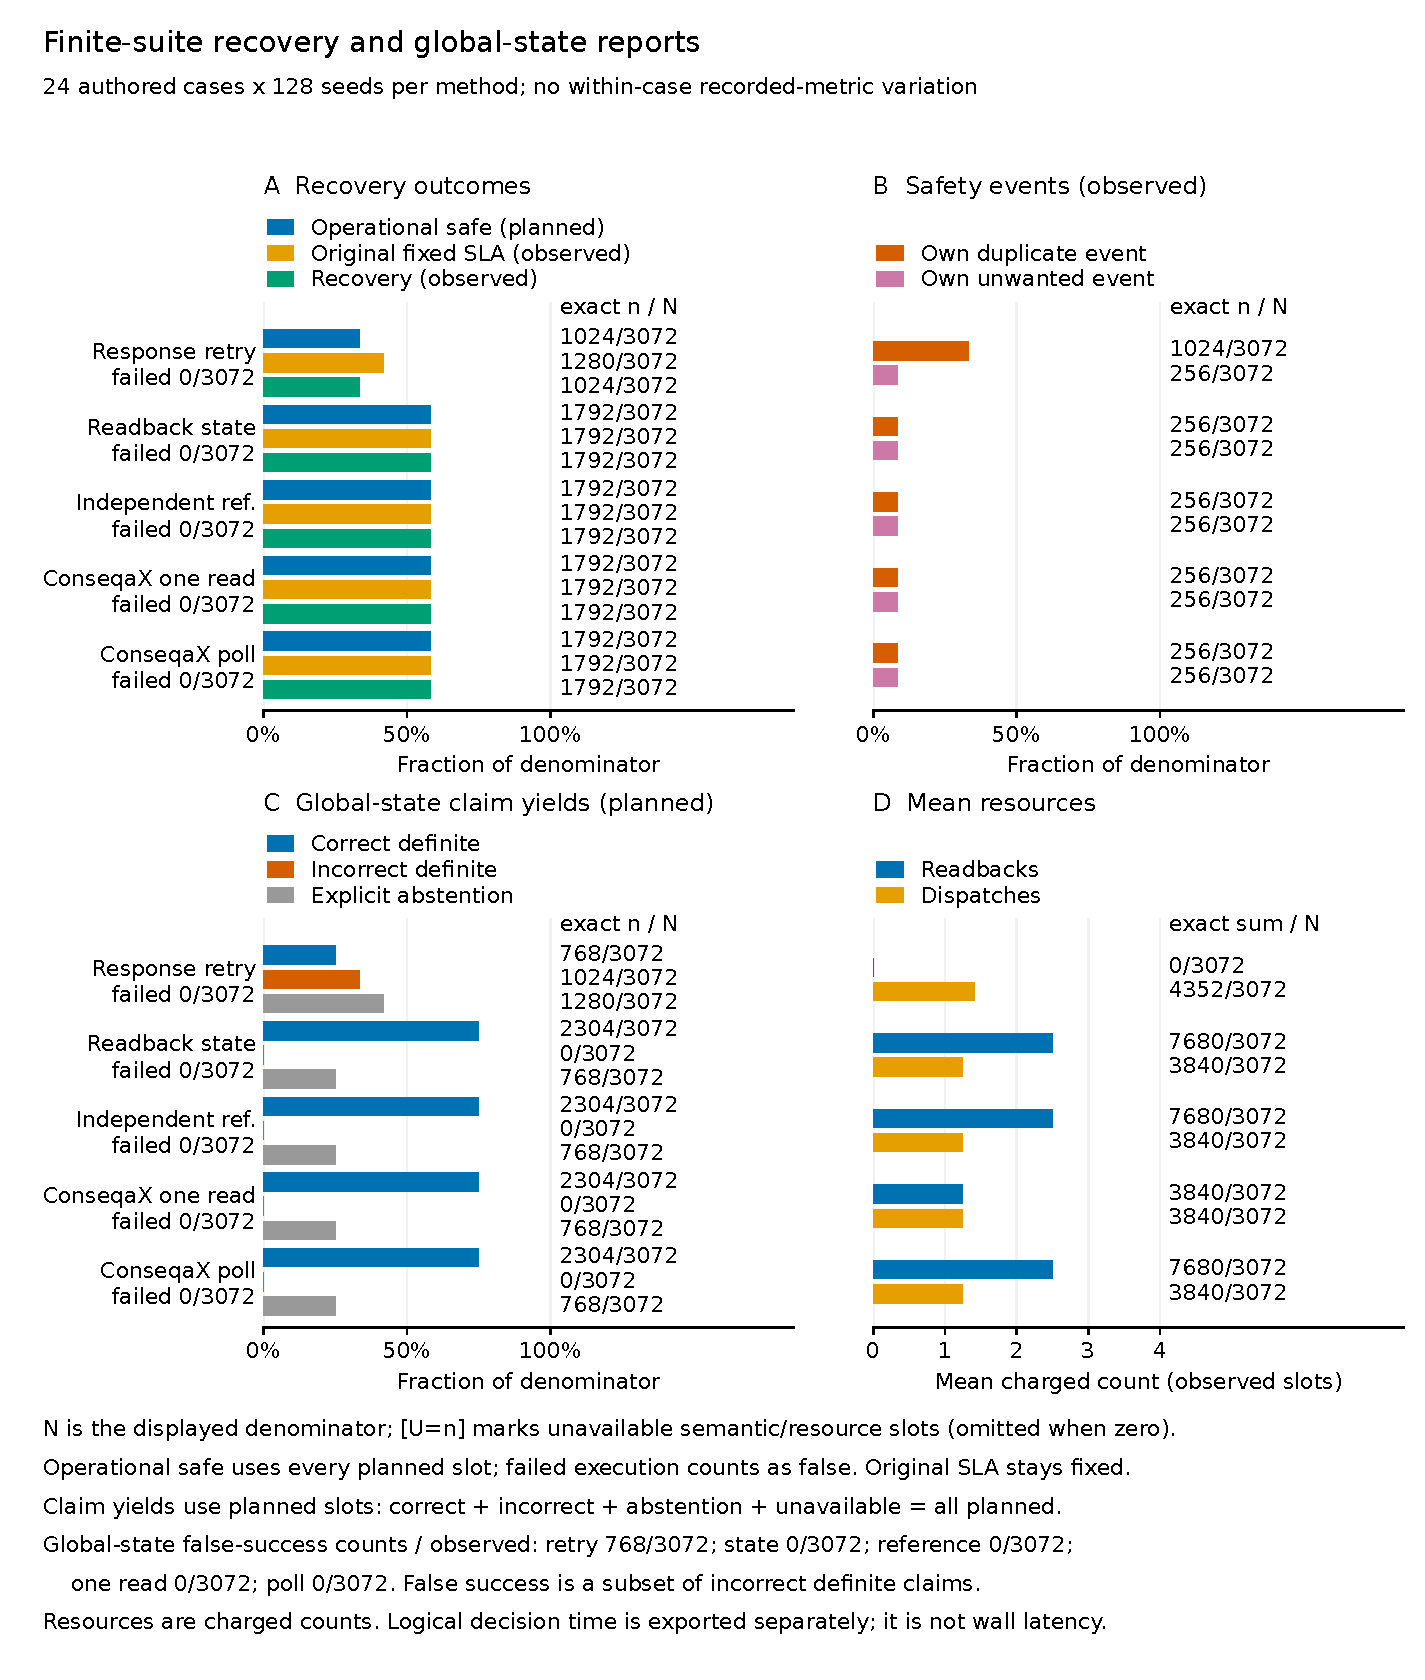
\includegraphics[width=\textwidth,height=0.89\textheight,keepaspectratio]{recovery-method-overview.pdf}
\caption{Study A: all five policies, exact denominators, own harmful events, global-state reporting, and read/dispatch costs. All recorded metrics were constant across seeds within each of the 24 authored cases. Reference independence concerns evidence arithmetic; application transitions and controller authorship are shared. Reporting correctness is distinct from physical recovery and evidence support.}
\label{fig:recovery-overview}
\end{figure*}

\begin{figure*}[t]
\centering
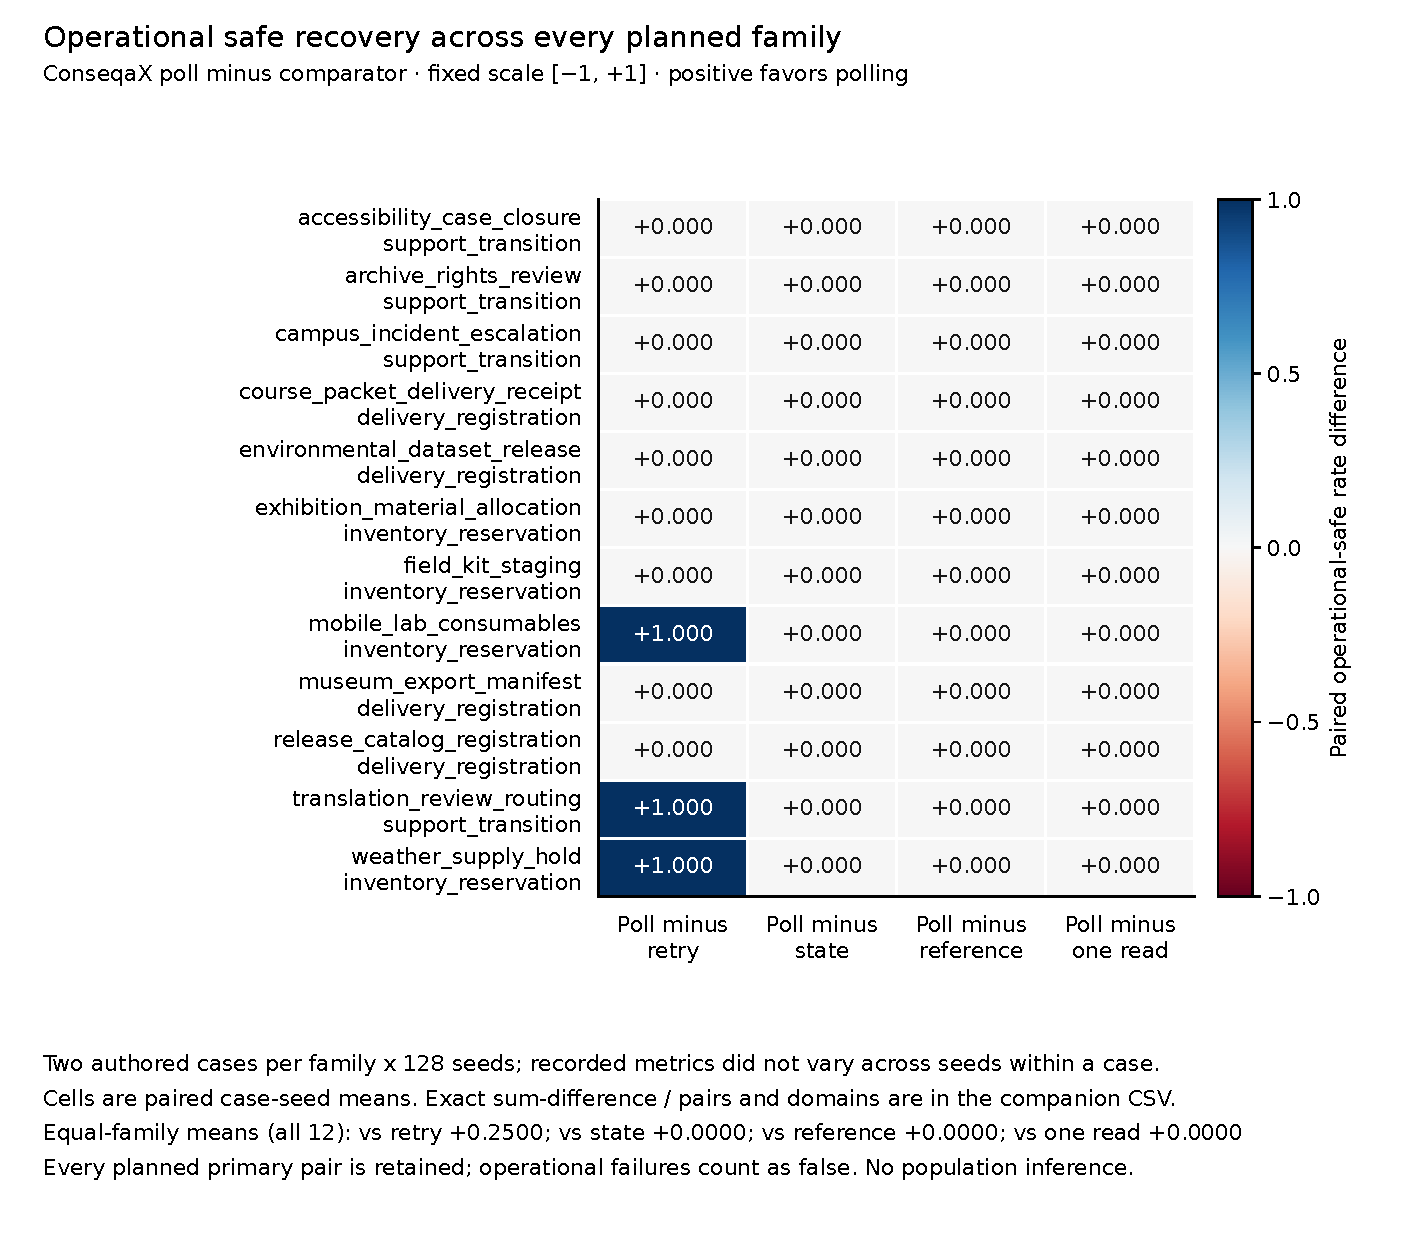
\includegraphics[width=\textwidth,height=0.76\textheight,keepaspectratio]{recovery-family-primary-contrasts.pdf}
\caption{Study A: every planned family's paired operational-safe difference, on a fixed $[-1,1]$ scale. Each family has two related cases and 128 seeds; repetitions added no recorded-metric variation. The equal-family difference is $+0.25$ against response retry and zero against all three readback comparators. These purposive families do not support task-population inference.}
\label{fig:recovery-families}
\end{figure*}

\subsection{Study B: controlled evidence availability}

Study A's coverage gap motivated a separate follow-up after its outcomes were known. We retained the byte-identical world, controllers, and evaluator, then froze a new complete factorial grid before collecting its own data. Source commit \texttt{\seqsplit{d805b3e3560c05ee0a7efd02a80fc18503c6ee05}}, protocol commit \texttt{\seqsplit{b937920469285cdd971783fa6cb33216a7e4da13}}, and protocol SHA-256 \texttt{\seqsplit{e874c6781aa0dbc8ef682ea0a8d37c25d73cc861dada05fd0379116d4a7f6584}} bind that design. This is a disclosed, post hoc motivated sensitivity experiment, rather than a new held-out corpus or replacement for Study A.

The 64 profiles cross readback lag $\{0,40,80,95\}$ ms with independently varied unavailable-until and incomplete-until times $\{0,170,210,250\}$ ms. Each profile repeats in the three domains at seed zero: 192 cases and 960 scheduled policy worlds. Here $D=100$, $H=150$, $R=250$, and $S=330$ ms; reads remain at $50,150,190,230$ ms. Every initial dispatch acknowledges at 2 ms and creates one correct effect at 10 ms. All arms share native idempotency. There are no external writes, removals, or wrong effects. This intentionally uniform physical-success design isolates evidence-window coverage and cost. Profiles are controlled mechanisms, and the three domains repeat them; neither 192 cases nor 960 worlds represent independent task samples.

All 960 worlds completed without failure. The separately implemented auditor verified 1,925 saved artifacts, queried all 960 SQLite snapshots, and agreed with the summary. Unlike Study A, the original collector produced its terminal manifest and receipt normally. All five policies dispatched once, achieved original and recovery satisfaction in 192/192 worlds, and had zero duplicate or unwanted events. Their physical effect histories agreed in every five-arm case. Thus the primary safe-recovery contrast is zero.

\begin{table*}[t]
\caption{Study B: exact finite-grid reports and read costs, 192 planned/completed worlds per policy. Every definite report is hindsight-correct in this uniform-success design. It cannot estimate the response policy's false-success risk. Linked abstention is distinct from state abstention.}
\label{tab:availability-results}
\centering\small
\setlength{\tabcolsep}{4pt}
\begin{tabular}{lrrrrr}
\toprule
Policy & State correct/planned & State unknown & Linked correct/planned & Total reads & Mean decision (ms) \\
\midrule
Response retry & 192/192 & 0/192 & 192/192 & 0 & 2 \\
Readback state & 81/192 & 111/192 & 0/192 & 741 & 224.375 \\
Separate reference & 81/192 & 111/192 & 81/192 & 741 & 224.375 \\
ConseqaX one final read & 3/192 & 189/192 & 3/192 & 192 & 150 \\
ConseqaX polling & 81/192 & 111/192 & 81/192 & 741 & 224.375 \\
\bottomrule
\end{tabular}
\end{table*}

The one-final-read policy resolved one of 64 profiles per domain; polling resolved 27, matching the prospectively specified timing calculation. The paired correct-state-yield increase is $78/192=26/64=0.40625$, shared by the reference and state-only readback. All 192 reference--polling pairs agreed on reports, endpoint vectors, dispatch decisions, and physical records. State-only differed from polling in 81 linked reports while preserving actions and physical outcomes. Polling used 741 reads versus 192 for one-final-read, or 3.859375 versus one per world; mean logical decision time increased by 74.375 ms. These are charged simulated reads and decision times, not production latency.

The full factor grid in Fig.~\ref{fig:availability-grid} shows the boundary: late opportunities help only when availability and completeness recover and the watermark reaches $H$. Lag 95 ms and either window persisting through 250 ms remain unresolved. The ACK-driven response policy reports all 192 successes correctly in hindsight with no read, since all effects are constructed to succeed. Its report arrives before the effect and without horizon-covering evidence; this experiment supplies no estimate of its risk in failing worlds. Together, the studies show conditional polling utility and its cost, with no package superiority over the equally informed reference, no additional recovery-action benefit, and no task-population inference.

\begin{figure*}[p]
\centering
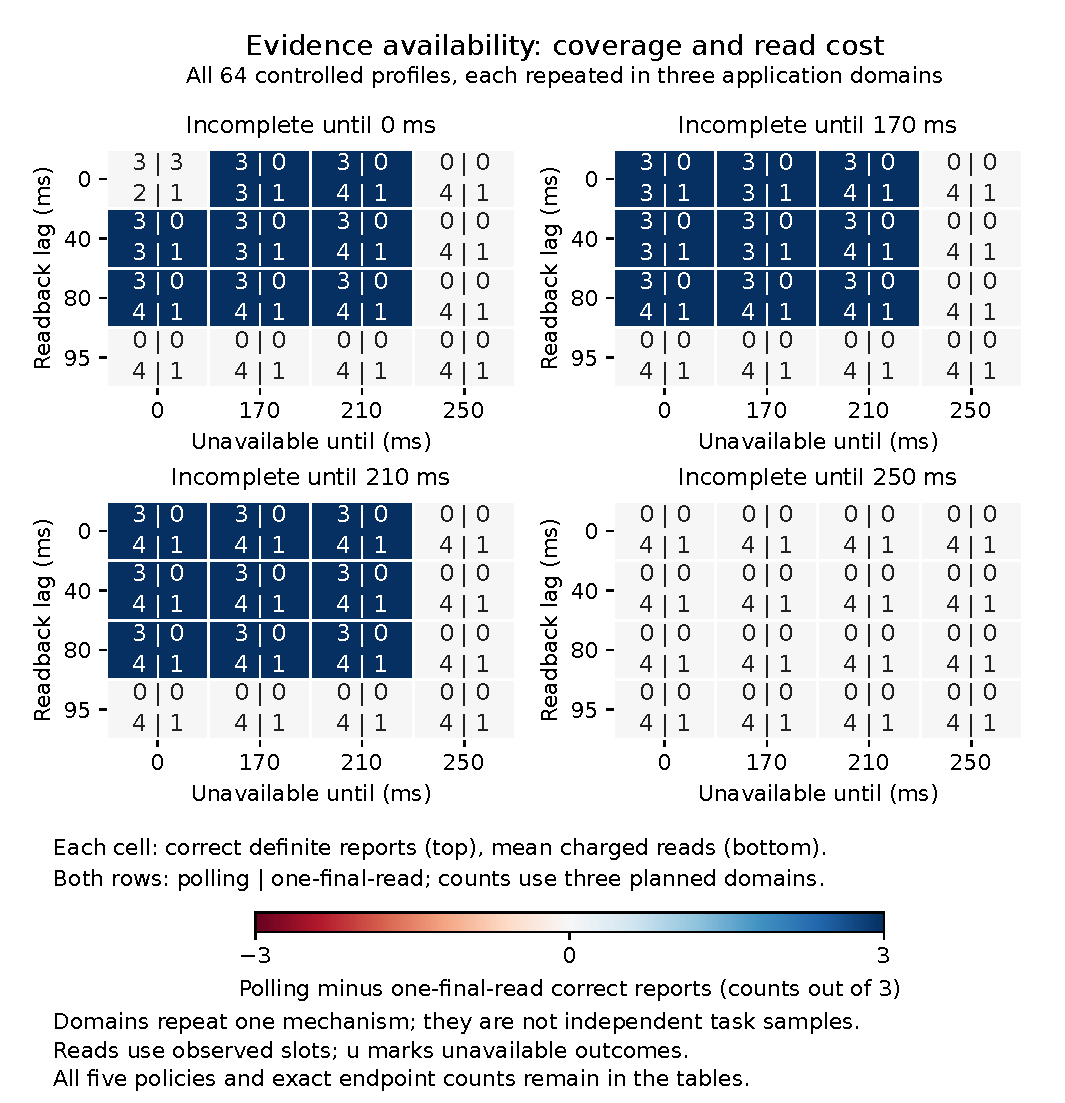
\includegraphics[width=\textwidth,height=0.76\textheight,keepaspectratio]{recovery-availability-grid.pdf}
\caption{Study B: all 64 controlled availability profiles, repeated across three domains. Actual report coverage and read costs are retained for polling and one-final-read. These paired conditions isolate evidence timing; every policy has identical successful physical outcomes, and the classical reference matches polling.}
\label{fig:availability-grid}
\end{figure*}



\section{External Native Fault-Benchmark Methods}
\label{sec:limbo}

The complete schedule, execution sources, native implementation, wheel and runtime identities for the separately declared follow-up were published before its generation at protocol commit \texttt{\seqsplit{8b25d4c7769c5c593333c9d3eeeceb8ae001dba4}}. The protocol SHA-256 is \texttt{\seqsplit{6d34556a03e9d738d11367a40d4812cb93168c82d3ae775ef76f1a4c48679541}}. All 96 planned follow-up dispositions are retained, including errors and unavailable grades. Source, model and resource bindings are part of the accompanying audit-linked artifact. The original cohort at protocol commit \texttt{\seqsplit{267cd1a3e846c46c009f20accbf302746e064875}} was interrupted after 6/96 native grades became available. Its original final collector seal and process terminal are unavailable. A separately dated postcollection preservation archive binds copied original bytes; replay reconstructs only available sealed child returns. The remaining dispositions stay unknown, including the interrupted child and every unstarted slot. No original exit status or interruption cause is invented. Both 96-slot cohorts remain in the paper and artifact. The host migration required explicit runtime-path repairs, a new private runtime binding and a change from Ollama 0.40.8 to 0.40.10. The follow-up was declared after access to the partial original data. It reuses the same weights, frozen scientific sources, task indices, fault assignments, arm order, control settings, limits and analysis. It is a distinct runtime condition, not a resume, successful-slot replacement or independently sampled replication. Its within-world contrasts are primary; cross-cohort outcomes and costs are descriptive and never pooled. The two planned cohorts still contain only 12 unique base instances.

\subsection{Benchmark, selection, and matched conditions}

The external environment is the author-maintained LIMBO sandbox
\cite{limbo,limbosource}, pinned to commit
\texttt{\seqsplit{2db09fba22a0572a70639162a808906409f612a8}}. This source pin
differs from its \texttt{v1.0} tag
(\texttt{\seqsplit{83c59e31f8477a5fb6f186dfcc9f3d10fa336b8a}}); our executions
are not a reproduction of the preprint's released episode corpus. Native task
construction, service implementation, fault injection, policy prompts, tool
schemas, final settlement and grading remain unchanged. We use the minimal
native agent loop through a scoped policy-factory extension, rather than the
stock parallel runner and its retry/resume behavior. All services are simulated;
no production service write or real human intervention is involved.

The frozen schedule selected one parameterized base instance from each of
the 12 external templates across billing, data, deploy, mail, social and
tickets. Instance indices are hash-selected from the declared seed and index
salt, excluding development indices. A trusted extractor releases only
template/domain identifiers, focal-write names and public affordances for
selection; task instructions, targets, setup values and grader outcomes do not
enter the selection rule. Each base instance has a clean condition and one
compatible fault condition. Metadata-based balancing and hash tie-breaking
cover pre-dispatch timeout, post-commit timeout, late commit, heavy-tailed late
commit, partial-batch timeout and duplicate delivery; the batch-capable template
is reserved for the partial-batch condition. This is finite purposeful coverage,
not a random task sample or an exhaustive fault cross-product.

Four arms defined 24 task/fault conditions and 96 planned execution slots on
12 base instances. Rotating arm order balanced execution positions. Arms share
the native world within a condition, public capabilities, neutral tool
documentation, default instruction and resource limits. Clean and fault
conditions share base task parameters, but the native world RNG seed depends
on fault mode; they are not identical random worlds. The primary contrasts are
between arms within each world.

\begin{table}[t]
\caption{Frozen native comparison. The SDK arm preserves the supplied
strong guard's control law; it is a receipt-integration comparison.}
\label{tab:limbo-arms}
\centering\small
\setlength{\tabcolsep}{3pt}
\begin{tabular}{p{0.25\columnwidth}p{0.65\columnwidth}}
\toprule
Arm & Execution rule \\
\midrule
\texttt{vanilla} & Unchanged native direct tool dispatch. \\
\texttt{sdk\_retry3} & Unchanged native transparent retry rule: up to three
automatic retries after an initial retryable failure, with native backoff. \\
\texttt{guard} & Unchanged native strong guard: supported key insertion,
consistency-aware verification, partial-batch recovery and repeat suppression. \\
\texttt{conseqax\_guard} & The same strong guard consuming statuses reconstructed
from actual ConseqaX 2.1.1 receipts. \\
\bottomrule
\end{tabular}
\end{table}

\begin{figure*}[t]
\centering
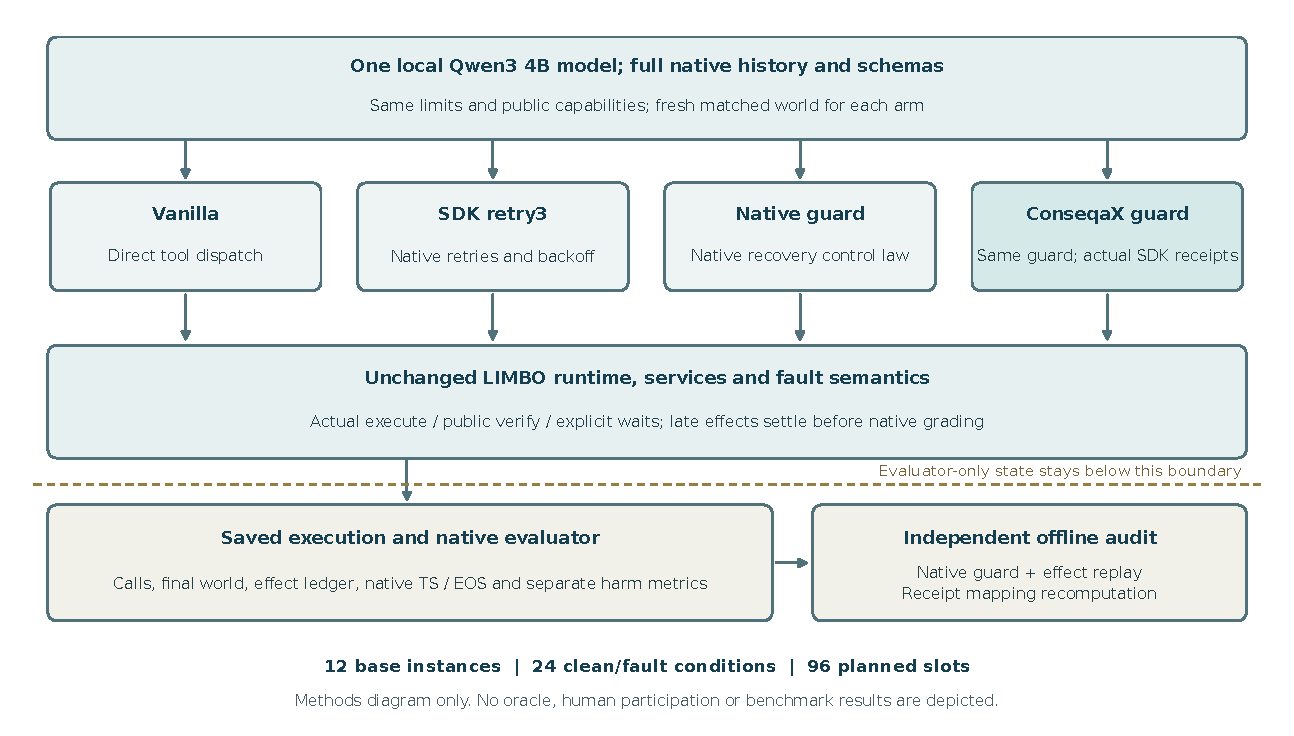
\includegraphics[width=\textwidth,height=0.67\textheight,keepaspectratio]{limbo-native-methods.pdf}
\caption{Native public-information boundary and four matched conditions. The package arm preserves the supplied strong guard while consuming actual SDK receipts. Only public reports enter the receipt path; targets, faults, ledgers and native grades remain evaluator-only. Offline replay checks behavior and receipt mappings, not an independently operated service or SDK re-execution.}
\label{fig:limbo-methods}
\end{figure*}

\subsection{Actual SDK path and public-information boundary}

Qualification evidence is separated from measurement. Preserved excluded autonomous native executions validated normal baseline/guard returns under the historical runtime; a separately scripted repeated-proposal fixture exercised the actual SDK receipt path without model generations or a native task grade. Relocated readiness retained those historical executions and added current-runtime full-schema render/token parity and a two-call task-independent structured-tool roundtrip. Historical executions are not relabeled as current-runtime trajectories, and fixture receipts do not enter measured counts. Measured follow-up activation comprised 3 audited receipts in 3/24 planned SDK episodes; 24/24 had complete audited accounting. The auditor checks saved receipt mappings and native behavior; it does not independently re-execute the SDK or authenticate a production service.

The package arm invokes the installed 2.1.1 wheel, bound together with all
54 installed payload files, through a custom public-report verifier. Every
actual native \texttt{verify(..., truth=False)} result produces a typed action,
contract, observation and verification receipt. After receipt-binding checks,
the guard consumes the reconstructed native status/detail. It does not bypass
the receipt with a raw status. A clean first acknowledgement need not invoke
verification and can therefore produce zero receipts. No extra read or prompt
intervention is introduced solely to create a receipt.

Package inputs contain only copied public arguments, contract metadata,
timestamps and the returned public verification report. Task targets, pending
requests, fault plans, effect ledgers, final grades and raw service callbacks
remain evaluator-only. A narrow facade supplies the original guard's admitted
runtime accesses; it does not expose the complete world. This is a trusted-code
information boundary, not an operating-system sandbox against hostile
introspection. The original native baseline policies retain their original
runtime. \texttt{human\_available=False} disables the simulated operator in all
arms; attempted escalation can still fail and advance virtual time.

Native \texttt{found} maps to a satisfied current-visible-match predicate and
\texttt{absent} to its violation. Partial, unverifiable and other unresolved
reports map to unknown while retaining their exact native status/detail for
the guard. Origin is always unknown. These are current public-report receipts,
not evaluations by the built-in temporal \texttt{RecordVerifier}. They establish
neither durable settlement, action ownership, a retry-safe terminal request nor
universal exactly-once execution. The native verifier is the supplied simulator
abstraction, not an independently operated second service.

Invented-world integration checks compare the native and package guard on
identical proposals, actual calls, public reports, interventions, waits and
settled worlds. The external comparison retained this declared
control law under autonomous model proposals. Agreement is expected when the
shared control law is preserved; it is not algorithmic superiority. Native
guard limitations, including possible late-commit ambiguity and later repeated
same-intent dispatch, remain part of the comparison.

\subsection{Local model, transport, and fixed resources}

The frozen runtime used Qwen3-4B-Instruct-2507 \cite{qwenmodel}, the exact
\texttt{\seqsplit{qwen3:4b-instruct-2507-q4\_K\_M}} quantization distributed by
Ollama \cite{ollamaqwen}, served
locally by version 0.40.10 \cite{ollamaruntime}. The frozen artifact binds
the full model-blob digest, alias manifest, server and runner executable hashes,
process identities and creation times, interpreter and dependency versions.
The frozen configuration was one 8,192-token cache slot, q8 KV cache,
temperature zero, seed 1701 and at most 512 output tokens per permitted request.
The seed is a disclosed transport extension; it does not establish bitwise
repeatability. There is one model role and no hosted inference.

The client retains the native chat-message construction and response parser.
Before every generation it compares the complete locally predicted prompt with
the live server-rendered bytes and all runtime token IDs. Full history and tool
schemas are retained, with the output allowance and 64-token reserve included
in the context gate. A disclosed compatibility correction elides only literal
default-true \texttt{additionalProperties} fields from copied typed-schema
nodes in the offline predictor; actual HTTP schemas remain unchanged.
Unsupported constrained forms are refused rather than silently weakened.

Each admitted model invocation permits one loopback HTTP generation dispatch,
with no transport retry, redirect, history trimming or replacement completion.
Exact request/response bytes, failed sends, parsing failures and available usage
are retained. Missing usage remains unknown, and cached input tokens are not
added again to input totals. The frozen shared ceilings were 16 model
invocations, 16 proposed native tool calls, 1,200 seconds per request and
7,200 seconds per trajectory. An additional call refused at the invocation cap
is recorded separately and performs no HTTP generation. Automatic tool retries
remain visible actual work rather than model proposals.

Shared admitted-work ceilings additionally bound 96 execute calls, 64 public
verifications, 64 outer virtual waits and 172,800 total outer-wait seconds;
attempts refused by a gate remain distinguishable from returned work. Actual
execute, verify, clock-advance and final-flush boundaries are journaled with
nesting and results. Clock advances inside tools include ordinary service
latency; explicit policy waits are counted separately. Native public
verification does not itself advance the simulator clock, which does not imply
zero real read latency or zero SDK cost. Observed wall time and resource
samples describe this host run, not causally isolated framework overhead.

\subsection{Native endpoints, audit, and analysis}

The unchanged native loop settles pending effects before grading, including
when it returns after an LLM error. Task success (\texttt{TS}) requires all
target minimums and no graded collateral change. Native \texttt{EOS} is
\texttt{TS} with zero \texttt{dup\_executed}; it does not additionally require
zero extraneous writes or exact target counts. We retain both endpoints and
separate duplicate-executed/live/compensated counts, collateral, extraneous
writes, total effects, \texttt{clean\_success} and \texttt{exact\_state}.
\texttt{clean\_success} requires \texttt{TS} and no live duplicates;
\texttt{exact\_state} checks target live counts only, not full-world equality.

The duplicate counters are domain-qualified. Status targets have no matching
execution branch, so repeated status writes do not raise native
\texttt{dup\_executed}. Matching upsert creation counts are capped at final
matching live count, whereas refund execution counts are not capped.
\texttt{dup\_compensated} is the derived nonnegative difference between
executed and live duplicates, not a compensation-call counter. Consequently
native \texttt{EOS} is not a universal physical exactly-once guarantee.

The registered primary numerator counts independently replayed native
\texttt{TS}/\texttt{EOS} successes over every planned slot per arm. Operational
grade availability includes audited native error returns after settlement;
execution without native error is a separate secondary outcome. A missing grade
cannot earn primary success but is not assigned an invented semantic zero.
Failed, interrupted and unstarted slots retain their planned positions, with
no retry, resume, deletion or replacement.

A separately implemented offline auditor imports neither collector, package
policy, transport nor SDK. It reconstructs native model requests and parsed
responses, actual public calls, virtual waits, settlement, final world and RNG
state, ledger and every native grade field. The SDK arm is replayed through the
original native guard with the same episode identity, while receipt bindings
and public-status mappings are recomputed separately. This checks native
behavioral conformance and receipt arithmetic, not SDK re-execution or an
independent service verifier. Saved render/token proofs receive consistency
checks; the auditor does not independently rerun the tokenizer. Audit success
does not imply all planned executions returned or tasks succeeded. These are
automated checks within the same AI-assisted project, not external replication.

Analysis retained all planned slots and reports exact finite-suite counts,
within-world paired contrasts, per-template variation, assigned-fault strata,
grade/usage availability and actual costs. Fault triggering is a recorded
post-execution outcome, not an inclusion rule. Repeated arms and clean/fault
variants do not add independent tasks; no population confidence interval,
significance, equivalence or noninferiority claim follows from this selection.

\section{External Native Results}\label{sec:limbo-results}

The original interrupted cohort retains its full 96-slot denominator: 6 independently replayed grades, 0 native error returns among those grades, and 90 unavailable grades. Its all-planned counts are Vanilla TS/EOS 1/24 and 1/24; SDK retry TS/EOS 2/24 and 2/24; Native guard TS/EOS 1/24 and 1/24; ConseqaX guard TS/EOS 1/24 and 1/24. The original collector's final seal is unavailable; its audit binds a later copy-only preservation archive and does not manufacture missing terminal evidence. The separately published follow-up is the primary runtime condition below. Both cohorts reuse the same 12 base instances and 24 condition definitions; they are not pooled or counted as 192 independent tasks. Original interrupted cohort: audited\_native\_return 6; interrupted\_terminal\_unavailable 1; unstarted\_interruption 89. Follow-up cohort: audited\_native\_error\_return 3; audited\_native\_return 93.

% Derived separately from both complete 96-slot audited cohorts; no pooling.
\begin{table*}[t]
\caption{Both registered cohorts retain their full planned denominators. Started includes an interrupted child; graded includes independently replayed native error returns after settlement. Unknown grades remain unavailable. The follow-up uses the same 12 base instances and is not an independent task sample.}
\label{tab:limbo-cohorts}\centering\small\setlength{\tabcolsep}{4pt}
\begin{tabular}{llrrrrrrr}\toprule
Cohort & Arm & Planned & Started & Graded & Error returns & Unavailable & TS & EOS \\
\midrule
Original interrupted & Vanilla & 24 & 1 & 1 & 0 & 23 & 1 & 1 \\
Original interrupted & SDK retry & 24 & 2 & 2 & 0 & 22 & 2 & 2 \\
Original interrupted & Native guard & 24 & 2 & 2 & 0 & 22 & 1 & 1 \\
Original interrupted & ConseqaX guard & 24 & 2 & 1 & 0 & 23 & 1 & 1 \\
Follow-up & Vanilla & 24 & 24 & 24 & 0 & 0 & 21 & 16 \\
Follow-up & SDK retry & 24 & 24 & 24 & 0 & 0 & 24 & 14 \\
Follow-up & Native guard & 24 & 24 & 24 & 1 & 0 & 21 & 16 \\
Follow-up & ConseqaX guard & 24 & 24 & 24 & 2 & 0 & 20 & 15 \\
\bottomrule\end{tabular}\end{table*}


The frozen external matrix comprised 12 base instances from 12 templates across six focal domains, each in a clean condition and one compatible assigned fault condition. Four arms produced 96 planned slots on 24 matched native worlds. These are 12 base instances, not 96 independent tasks. Independent replay established native grades for 96/96 slots, including 3 native error returns after native settlement; 0 grades were unavailable. An audited error return remains eligible for the physical endpoint; normal execution success is reported separately.

Assigned-condition results were Vanilla: clean TS/EOS 12/12 and 11/12, assigned-fault TS/EOS 9/12 and 5/12 (grades available 12/12 and 12/12); SDK retry: clean TS/EOS 12/12 and 11/12, assigned-fault TS/EOS 12/12 and 3/12 (grades available 12/12 and 12/12); Native guard: clean TS/EOS 12/12 and 11/12, assigned-fault TS/EOS 9/12 and 5/12 (grades available 12/12 and 12/12); ConseqaX guard: clean TS/EOS 11/12 and 10/12, assigned-fault TS/EOS 9/12 and 5/12 (grades available 12/12 and 12/12). Strata use the prospective assignment, irrespective of whether a policy triggered the fault. Base task parameters match between clean and fault conditions, but native random seeds depend on mode; these descriptive condition differences do not identify a fault-only causal effect.

Follow-up matched baseline contrasts over all 24 planned native worlds were Native guard minus Vanilla: TS numerator difference +0/24, both grades available 24/24 and at least one grade unavailable 0/24; EOS numerator difference +0/24, both grades available 24/24 and at least one grade unavailable 0/24. Native guard minus SDK retry: TS numerator difference -3/24, both grades available 24/24 and at least one grade unavailable 0/24; EOS numerator difference +2/24, both grades available 24/24 and at least one grade unavailable 0/24. These finite paired counts retain every unavailable pair; they are not population significance, equivalence or an independent recovery-algorithm claim.

The original six graded prefix slots, one interrupted slot and 89 unstarted slots do not support an efficacy comparison of that condition. Its 90 unavailable grades are not native failures.

\begin{table}[t]
\caption{Follow-up runtime condition. All-planned native results. Graded means an independently replayed native grade; it includes native error returns after settlement. Missing is not an invented semantic zero.}
\label{tab:limbo-results}\centering\small\setlength{\tabcolsep}{3pt}
% Generated from a sealed passed official audit; do not edit values by hand.
% Native EOS is domain-qualified; all-planned denominators include unavailable grades.
\begin{tabular}{lrrrrr}
\hline
Arm & $n$ & Graded & TS & EOS & Missing \\
\hline
Vanilla & 24 & 24 & 21 & 16 & 0 \\
SDK retry & 24 & 24 & 24 & 14 & 0 \\
Native guard & 24 & 24 & 21 & 16 & 0 \\
ConseqaX guard & 24 & 24 & 20 & 15 & 0 \\
\hline
\end{tabular}

\end{table}

The ConseqaX arm emitted 3 audited SDK receipts across 3/24 planned episodes with at least one receipt (24/24 episodes had complete audited accounting). The package consumes unchanged current public verification reports; clean first acknowledgments can therefore require no receipt. The independent auditor recomputes receipt mappings and replays the original native guard and physical effects, but does not independently re-execute the SDK. The integration implements the same recovery decisions as the strong native comparator, rather than a new recovery algorithm or a claim of causal origin.

For the native-guard versus ConseqaX-guard comparison, 24/24 matched worlds had both native grades available. Their TS booleans agreed in 23 and EOS booleans agreed in 23 of those worlds; 0/24 worlds had at least one unavailable grade. These are descriptive paired outcome agreements. Separately generated model trajectories need not coincide, and this finite matrix supports neither population equivalence nor algorithmic superiority.

Observed work totals were Vanilla: 151 execute attempts, 0 public verification attempts, 0 explicit wait attempts and 124 model generation dispatches from 24/24 slots with complete accounting; SDK retry: 157 execute attempts, 0 public verification attempts, 10 explicit wait attempts and 126 model generation dispatches from 24/24 slots with complete accounting; Native guard: 168 execute attempts, 3 public verification attempts, 0 explicit wait attempts and 156 model generation dispatches from 24/24 slots with complete accounting; ConseqaX guard: 159 execute attempts, 3 public verification attempts, 0 explicit wait attempts and 146 model generation dispatches from 24/24 slots with complete accounting. Incomplete slots may have additional unquantified work, so unavailable accounting is not zero. Boundary attempts are distinct from physical effects; nested clock advances include native tool latency and are not counted as explicit policy waits. Native virtual time and host wall time are separate costs.

Secondary native endpoint counts were Vanilla: clean-success 16/24 and exact-state 16/24; SDK retry: clean-success 14/24 and exact-state 14/24; Native guard: clean-success 16/24 and exact-state 16/24; ConseqaX guard: clean-success 15/24 and exact-state 15/24. Missing grades do not count as true; exact-state checks target counts only.

Across slots with complete audited accounting, journals retain 1249824 known input tokens and 51582 known output tokens, with 3 invocations lacking input usage and 3 lacking output usage. These are observed totals, not complete usage for slots without accounting. Cached input is already included in input totals. The artifact reports per-arm counts, assigned-fault/template/domain strata, paired contrasts and missingness without population significance or equivalence claims.

\begin{table*}[t]
\caption{Follow-up runtime condition. Observed native effect totals from graded slots only. Graded is the availability denominator, not a success count; unavailable effects are unquantified. Compensated is the native derived duplicate difference, not a count of compensation calls. Native domain qualifications apply.}
\label{tab:limbo-effects}\centering\small
\begin{tabular}{lrrrrrrr}\toprule
Arm & Graded & Dup. executed & Dup. live & Compensated & Collateral & Extraneous & Effects \\
\midrule
Vanilla & 24 & 8 & 8 & 0 & 0 & 0 & 89 \\
SDK retry & 24 & 14 & 14 & 0 & 0 & 0 & 100 \\
Native guard & 24 & 8 & 8 & 0 & 0 & 0 & 91 \\
ConseqaX guard & 24 & 8 & 8 & 0 & 0 & 0 & 88 \\
\bottomrule\end{tabular}\end{table*}

\begin{figure*}[t]
\centering
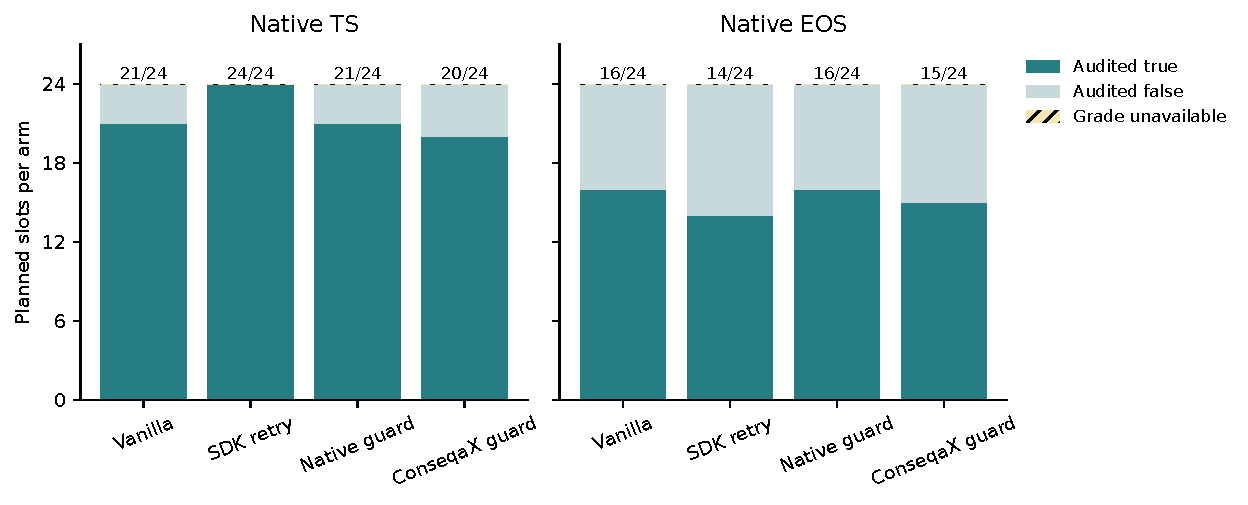
\includegraphics[width=\textwidth,height=0.67\textheight,keepaspectratio]{limbo-outcomes.pdf}
\caption{Follow-up runtime condition. Native TS/EOS true, false and unavailable grades over all 24 planned slots per arm. Error returns with audited settled grades remain physically assessable.}
\label{fig:limbo-outcomes}
\end{figure*}

\begin{figure*}[t]
\centering
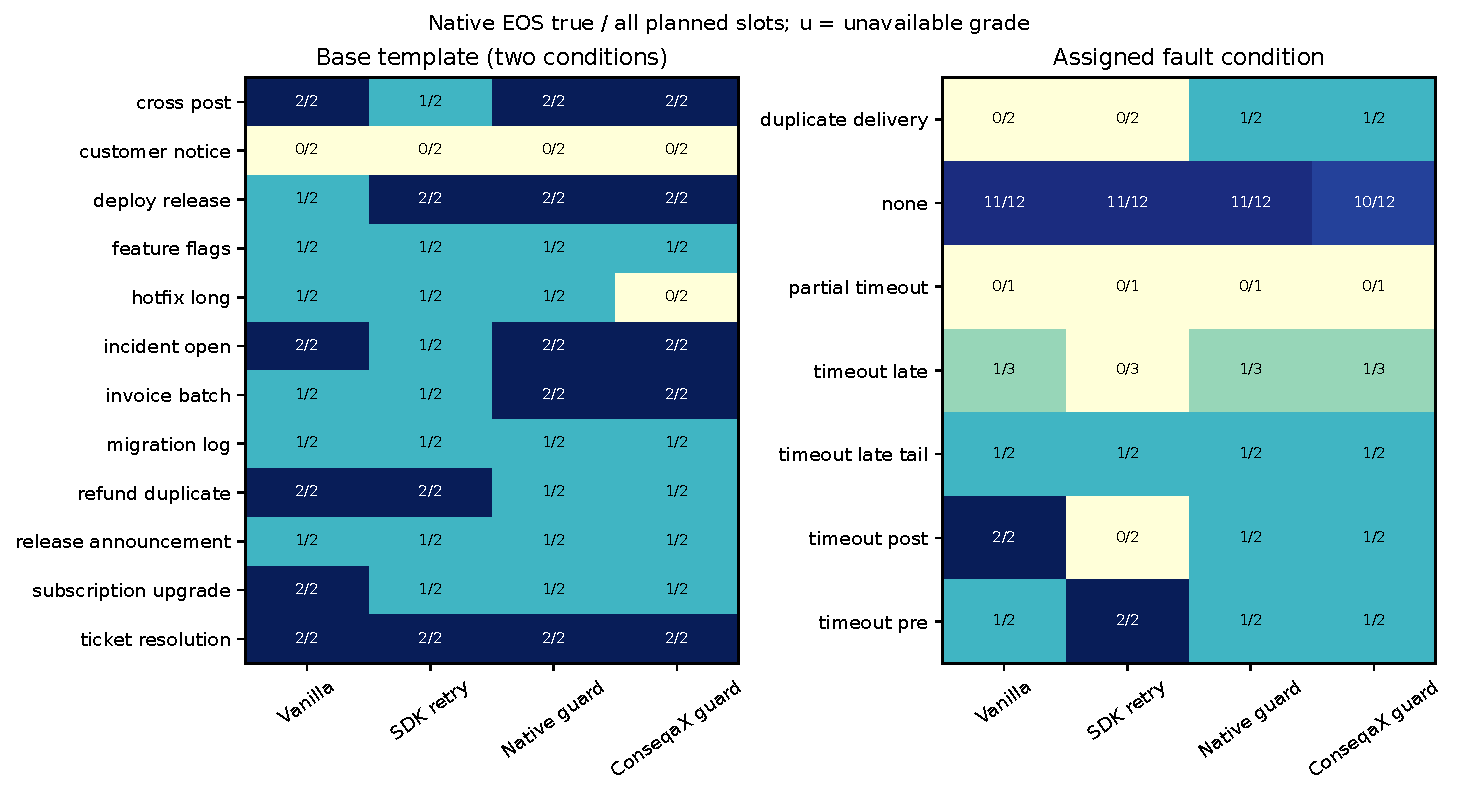
\includegraphics[width=\textwidth,height=0.67\textheight,keepaspectratio]{limbo-stratification.pdf}
\caption{Follow-up runtime condition. Native EOS true over all planned slots by base template and assigned fault. Unavailable grades remain marked. Strata are finite and descriptive; fault triggering is not an inclusion rule.}
\label{fig:limbo-stratification}
\end{figure*}

\begin{figure*}[t]
\centering
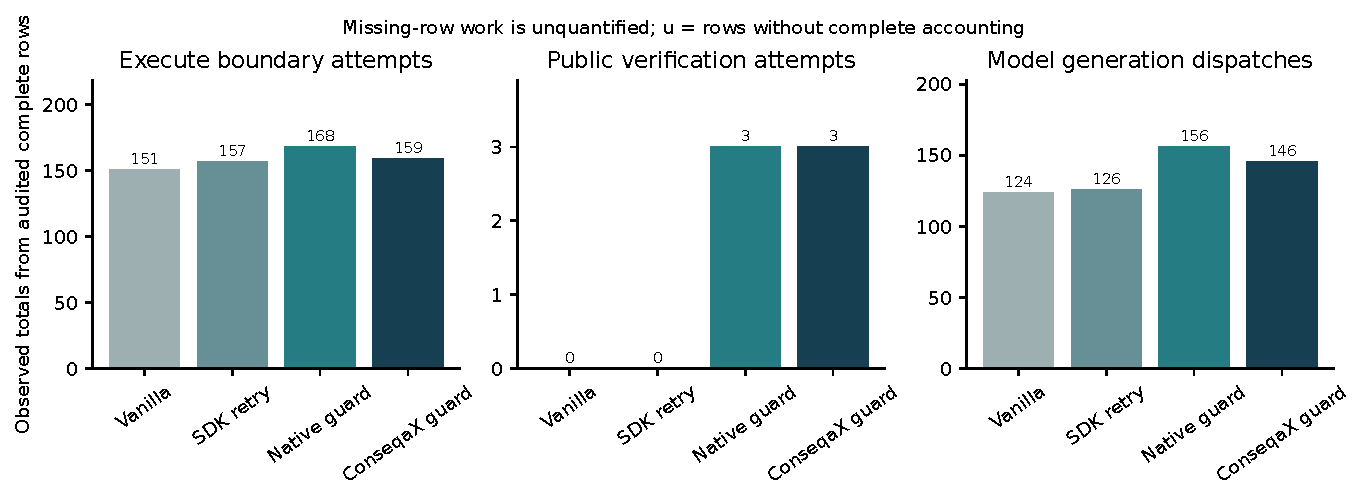
\includegraphics[width=\textwidth,height=0.67\textheight,keepaspectratio]{limbo-costs.pdf}
\caption{Follow-up runtime condition. Observed execute, public verification and model-dispatch totals from complete audited rows. Missing-row work is unquantified. Boundary attempts are not physical effect counts or isolated SDK overhead.}
\label{fig:limbo-costs}
\end{figure*}


\section{Supporting Evidence and Version Boundaries}

Earlier experiments corroborate narrower components without adding independent recovery families. Version 1.1.0 retained 503/504 factual-audit episodes across three small local models, with 72 unknown state reports; an 84-trace same-evidence judge made nine wrong among 60 definite state reports. Model-free tool transfer retained 656 cells and 900 operation captures, without autonomous reward. The native CAR bridge matched eligible point vectors in 640/1,024 paired groups; 384 were unavailable \cite{experimentartifact,carcode}. Version 2.0 offline migration preserved all 503 retained canonical conclusions while changing 275 diagnosis codes. The historical manuscript and versioned evidence ledger retain denominators, protocol deviations, and detailed results.

Studies A and B use selected ConseqaX 2.1.1 recording, contract, observation and built-in record-verification paths \cite{artifact}, together with explicit application polling and safety-gate code. The native LIMBO arm instead uses a custom verifier over current public reports; it does not exercise the temporal RecordVerifier. These studies do not evaluate the public blocking polling helper, composite/multiple-source verification, OpenTelemetry, unrelated SDK integrations or the full release surface. Historical 1.1.0 results and 2.0 migration retain their original versions; byte-identical numerical modules alone do not establish end-to-end version equivalence.

An earlier excluded airline development check used the native environment at revision 96a3ef92329baf908ffe9dfe188cea34e8701d2a. Its unwrapped execution returned 12 model completions and five tool calls but native reward 0 (DB 0; communication 1 was vacuous). Two guarded checks timed out at 600- and 1,200-second request limits, respectively, with no returned native grade and no SDK receipt. Their grades remain unavailable; they are excluded development evidence rather than paired comparative results. No official airline matrix was collected. Full original traces, partial failure audits and the historical manuscript retain these limitations.

\section{Discussion and Limitations}

An evidence protocol is useful only under meaningful source and operation semantics. A watermark covers history through a declared time; finite auditing through $S$ cannot prove absence of all future effects. Provider deduplication or terminal resolution is supplied equally to every arm, not created by verification. Concurrent external actors remain a distinct source of harmful global count changes. These assumptions constrain any recovery conclusion.

Strong-reference parity should be interpreted directly. Separate arithmetic reduces reliance on one verifier implementation, but a shared controller author and application state machine can preserve shared mistakes. The saved-artifact auditor uses separate code, while its author also implemented the controllers; this is not external replication. Exact agreement on this suite is neither superiority nor a proof of general safety. Advantages over response or state ablations must identify the omitted evidence and the precise claim or decision it changes. If provenance changes only reporting, that is the measured boundary; a causal action benefit cannot be inferred.

The controlled recovery corpus is small, purposive, AI-authored, and implemented on one local substrate. Three record domains broaden application vocabulary and predicate use without establishing transfer to independent services. Repeated timing seeds cannot repair this external-validity gap. Deterministic policies exercise recovery logic, not language understanding, user negotiation, planning, provider authentication, or autonomous tool selection. These data can characterize a conditional decision boundary; they cannot establish general autonomous-agent improvement or effectiveness across independently operated services.

Evaluation uses executable application contracts, effect-ledger ground truth, and separately implemented automated checks. No participant study or annotation study is part of this paper; interpretability, preference, rationale quality, and user trust are not measured. Automated cross-checks can expose implementation or arithmetic inconsistencies, but cannot establish that an external adapter's source-admission declarations or provider guarantees are true. That requires objective validation against the service's actual semantics and independently retained effects.

The external native study exercises ambiguous commits in authored LIMBO tasks with unchanged service semantics and native grading. It remains one 4B quantized local model, one declared seed, one base instance per template and one compatible assigned fault per template, rather than an exhaustive fault cross-product or a task-population sample. The follow-up condition was frozen after observing partial original results and repairing runtime paths after host migration; it is not an unseen replication or a replacement of the original. Both full 96-slot cohorts are retained separately on the same 12 instances. The original has 6/96 audited grades. Follow-up native grades are available in 96/96 planned slots, including 3 audited error returns after settlement; unavailable grades do not become semantic failures. The guard comparison uses the same control law; descriptive outcome agreement is not population equivalence. Native status/upsert duplicate accounting and target-scoped exact-state checks limit exactly-once interpretations. Serial host wall time, cache and shared load do not isolate SDK overhead. Independently operated service validation, broader model/task sampling and external replication remain outside these findings.

\section{Conclusion and Artifact Availability}

ConseqaX exposes inspectable boundaries between acknowledgements, admitted evidence, temporal state, operation-linked origin and explicitly unknown conclusions. The controlled studies show when polling improves report yield at additional cost and when it adds no benefit; the equally informed reference shares its gains. The 12-instance external native follow-up matrix retains all 96 planned dispositions and 96/96 audited grades: Vanilla TS/EOS 21/24 and 16/24; SDK retry TS/EOS 24/24 and 14/24; Native guard TS/EOS 21/24 and 16/24; ConseqaX guard TS/EOS 20/24 and 15/24. Its SDK condition emits 3 audited receipts in 3/24 planned episodes while preserving the supplied strong guard. The original interrupted cohort retains 6/96 audited grades and every unknown disposition separately; the same 12 instances are reused. These finite findings support an executable protocol and observed integration/coverage/cost tradeoffs rather than algorithmic superiority or universal exactly-once execution.

Studies A/B and both native runtime conditions retain the 2.1.1 package pin; the 2.1.2 distribution was released on 20 October 2026. The accompanying artifact binds protocols, exact source/runtime/wheel identities, planned schedules, dispositions, saved evidence, audits, analysis and deviations. The public repository is \url{https://github.com/Devrajsinh-Jhala/consequa-x}. A DOI-backed immutable archive has not been established. Historical replay, model, transfer and migration evidence retains its original targets and versions. No real payment or production-service write is part of these experiments. The evaluated and later release records are cited separately \cite{artifact,currentrelease}.

\section*{AI Assistance and Verification Disclosure}

Generative AI assisted software development, case creation, source inspection, automated artifact checking, and manuscript drafting. Separate AI authorship and saved-artifact audits do not constitute external replication. No participant or annotation study was conducted. The author is responsible for the manuscript and venue-required disclosure.

\FloatBarrier
\balance
\begin{thebibliography}{99}
\bibitem{helland}
P. Helland, ``Idempotence Is Not a Medical Condition,'' \emph{Communications of the ACM}, vol. 55, no. 5, pp. 56--65, 2012, doi: 10.1145/2160718.2160734.
\bibitem{vogels}
W. Vogels, ``Eventually Consistent,'' \emph{Communications of the ACM}, vol. 52, no. 1, pp. 40--44, 2009, doi: 10.1145/1435417.1435432.
\bibitem{verified} I. K. Mansoor, A. Phadke, and P. Rana, ``Verified Tool Calls
Improve LLM Agent Reliability Under Non-Atomic Failures,'' arXiv:2608.02645,
v1, Jul. 2026. [Online]. Available: \url{https://arxiv.org/html/2608.02645v1}
\bibitem{operability} Z. Wang, ``Callability Is Not Operability: Controlled
Interface Interventions for LLM Agents,'' arXiv:2608.23628, v2, Aug. 2026. [Online]. Available: \url{https://arxiv.org/html/2608.23628v2}
\bibitem{agenttool}
A. Trofimov and B. Novikov, ``When Tool Calls Succeed but Workflows Fail: Anomalies at the Agent-Tool Boundary,'' arXiv:2609.15397v1, Sep. 2026. [Online]. Available: \url{https://arxiv.org/html/2609.15397v1}
\bibitem{limbo}
J. Li, ``Where Does Exactly-Once Live? Model, Harness, and Tool-Contract Effects on Duplicate Side Effects in LLM Agents,'' arXiv:2609.29095v1, Sep. 2026. [Online]. Available: \url{https://arxiv.org/html/2609.29095v1}
\bibitem{artifact} D. Jhala, ``ConseqaX,'' MIT Python distribution,
ver. 2.1.1, Oct. 19, 2026. [Online]. Available:
\url{https://pypi.org/project/consequa-x/2.1.1/}
\bibitem{prov}
L. Moreau and P. Missier, Eds., ``PROV-DM: The PROV Data Model,'' W3C Recommendation, Apr. 30, 2013. [Online]. Available: \url{https://www.w3.org/TR/2013/REC-prov-dm-20130430/}
\bibitem{car} J. Shah, ``Causal Agent Replay: Counterfactual Attribution for
LLM-Agent Failures,'' arXiv:2606.08275, v1, Jun. 2026.
\bibitem{pccc} R. Meng, ``Policy-Conditioned Counterfactual Credit for Verifiable
Reinforcement Learning of Long-Horizon Language Agents,'' arXiv:2606.05263, v1,
Jun. 2026.
\bibitem{causalloss} A. Sharma, ``CausalLoss-Fin: Attributing Financial-Agent
Loss to Decisions and Infrastructure Faults,'' arXiv:2609.25960, v1, Sep. 2026.
\bibitem{appworld}
H. Trivedi \emph{et al.}, ``AppWorld: A Controllable World of Apps and People for Benchmarking Interactive Coding Agents,'' in \emph{Proc. 62nd Annu. Meeting Association for Computational Linguistics}, vol. 1, 2024, pp. 16022--16076, doi: 10.18653/v1/2024.acl-long.850.
\bibitem{toolsandbox}
J. Lu \emph{et al.}, ``ToolSandbox: A Stateful, Conversational, Interactive Evaluation Benchmark for LLM Tool Use Capabilities,'' in \emph{Findings of the Association for Computational Linguistics: NAACL 2025}, 2025, pp. 1160--1183, doi: 10.18653/v1/2025.findings-naacl.65.
\bibitem{taubench}
S. Yao, N. Shinn, P. Razavi, and K. Narasimhan, ``$\tau$-bench: A Benchmark for Tool-Agent-User Interaction in Real-World Domains,'' arXiv:2406.12045v1, 2024. [Online]. Available: \url{https://arxiv.org/html/2406.12045v1}
\bibitem{tau3tasks}
Sierra Research, ``tau2-bench: Maintained retail and airline task corpus,''
MIT software, commit 96a3ef92329baf908ffe9dfe188cea34e8701d2a, 2026.
[Online]. Available:
\url{https://github.com/sierra-research/tau2-bench/tree/96a3ef92329baf908ffe9dfe188cea34e8701d2a}
\bibitem{tau3eval}
Sierra Research, ``Native environment evaluator,'' tau2-bench, same pinned
commit, 2026. [Online]. Available:
\url{https://github.com/sierra-research/tau2-bench/blob/96a3ef92329baf908ffe9dfe188cea34e8701d2a/src/tau2/evaluator/evaluator_env.py}
\bibitem{experimentartifact} D. Jhala, ``Consequa-X,'' MIT Python distribution,
ver. 1.1.0, Oct. 17, 2026. [Online]. Available:
\url{https://pypi.org/project/consequa-x/1.1.0/}
\bibitem{carcode}
J. Shah, ``Causal Agent Replay,'' software ver. 0.2.0, commit
db90fa28b97164c35e7c524e4597b8cbdb3035af, 2026. [Online]. Available:
\url{https://github.com/jaineet17/causal-agent-replay/tree/db90fa28b97164c35e7c524e4597b8cbdb3035af}
\bibitem{currentrelease} D. Jhala, ``ConseqaX,'' MIT Python distribution,
ver. 2.1.2, Oct. 20, 2026. [Online]. Available:
\url{https://pypi.org/project/consequa-x/2.1.2/}
\bibitem{limbosource}
J. Li, ``LIMBO: Benchmark code, harness adapters and episode traces,'' MIT software, commit \texttt{\seqsplit{2db09fba22a0572a70639162a808906409f612a8}}, 2026. [Online]. Available: \url{https://github.com/jaxblack/limbo-bench/tree/2db09fba22a0572a70639162a808906409f612a8}
\bibitem{qwenmodel}
Qwen Team, ``Qwen3-4B-Instruct-2507,'' official model card, Apache 2.0. [Online]. Available: \url{https://huggingface.co/Qwen/Qwen3-4B-Instruct-2507}
\bibitem{ollamaqwen}
Ollama, ``qwen3:4b-instruct-2507-q4\_K\_M,'' Q4\_K\_M model distribution. [Online]. Available: \url{https://ollama.com/library/qwen3:4b-instruct-2507-q4_K_M}
\bibitem{ollamaruntime}
Ollama, ``Ollama,'' software vers. 0.40.8 and 0.40.10. Exact evaluated executable bytes are bound separately by cohort. [Online]. Available: \url{https://github.com/ollama/ollama/releases}
\end{thebibliography}
\end{document}
